\chapter{Experimental Postmarks}
\begin{marginfigure}
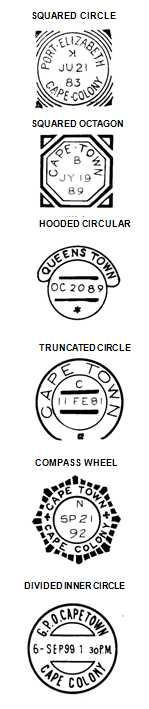
\includegraphics[width=.85\textwidth]{../cape-of-good-hope/experimental.jpg}
\caption{Experimental postmarks of the Cape of Good Hope.}
\end{marginfigure}	
Between the years 1882 and 1900 six handstamp designs were issued on  	 
what appears a highly selective basis. Their main characteristic 
being their unusual design. The purpose of them being issued was 
to find a datetamp that could be used for simultaneous defacing 
and dating of letters. The majority of them were only used at the General 
Post Office in Cape Town.  Others had limited distribution. 
The Squared Circle was the exception having been issued to some 
55 different post offices.


These handstamps can be classified as follows:

   
\begin{enumerate}
\item The Squared Circle Datestamp of 1882
\item The Squared Octagon Datestamp of 1887
\item The Hooded Circular Datestamp of 1888
\item The Truncated Circle Datestamp of 1890
\item The Compass Wheel Datestamp of 1891
\item The Divided Inner Circle Datestamp of 1898
\end{enumerate}

I found the inclusion of the Divided Inner Circle Datestamp necessary - 
although authors such as Goldblatt and Jurgens do not classify 
it as an experimental datestamp  as it has all the characteristics 
of an unusual design, limited distribution and relatively short life. 
The exhibit attempts to classify, hereto all the types and varieties 
as well as to present a chronological map of their usage and 
distribution and to record earliest and latest used example.

Their use was mostly deducted as a result of this exhibit and is 
summarised as follows:



\begin{enumerate}
\item The Squared Circle Datestamp of July 1882-Union Period
\item The Squared Octagon Datestamp of May 1888-1890
\item The Hooded Circular Datestamp of 1888-1890
\item The Truncated Circle Datestamp of 1890-1892
\item The Compass Wheel Datestamp of March 1892-1893
\item The G.P.O. Squared Circle datestamp 1894-1898
\item The Divided Inner Circle Datestamp of Jun 1898-1901
\end{enumerate}

The exhibit is mostly based mostly on the James Perkins correspondence 
where material was adequate in my collection to form a coherent study with very 
little gaps. Now and then I have used colour prints of back of postcards and letters. 
This was intended to give the reader a flavour of the times when these 
postmarks were used.

                                                                                                                                              


 

 
                                